\documentclass[letterpaper]{article}
\usepackage{natbib,reddit-sa}
\usepackage{filecontents,lipsum}
\usepackage{array}
\usepackage[obeyspaces]{url}
\usepackage{graphicx}

\makeatletter
\renewcommand{\fnum@figure}{Fig. \thefigure}
\makeatother

\title{2016 U.S. Presidential Election - Reddit Comment Temporal and Sentiment Analysis}
\author{Connor Griep$^{1}$, Jacob Shiohira$^{1}$, \and Jacob Warner$^{1}$ \\
\mbox{}\\
$^1$University of Nebraska-Lincoln, $1400$ R St, Lincoln, Nebraska \\
\mbox{}\\
connorgriep@gmail.com \\
jacob.shiohira@huskers.unl.edu \\
jwarner@huskers.unl.edu }


\begin{document}
\maketitle

\section{ABSTRACT}
The $2016$ presidential election was one of the most heated elections to date. The tone of the election campaign was generally characterized as divisive and negative, with both candidates surrounded with immense controversy. There was no way that both sides were going to be satisfied, but there is not a definitive source saying how the general population reacted to the events of the election. 

Reddit is a combination of social media, news sites and message boards, creating a unique community driven by engaging content. The platform is one of the best places to find authentic discourse, as people are looking to engage in discussion. The anonymity aspect of the platform guarantees people are free to speak their true feelings since their accounts are not necessarily tied to their name, like Facebook or LinkedIn. Further, it is rich in information about the public’s attitudes and feelings with respect to almost any topic, including politics. The election of the president is one of the most important events in the U.S. Thus, we believed Reddit to be a fascinating source to indicate America's feelings throughout the election process.

The comments from two weeks before and two weeks after the day of the election were analyzed for both sentiment and emotion. The resulting classifications were then aggregated in various visualizations to better find and understand any trends that developed throughout the election. A further investigation of the results can be found in the results section.

% ------------------------------------

\section{1 INTRODUCTION}

Reddit, a social media platform, has an active political community that is rich in information about the public's attitudes and feelings towards political topics and candidates. This project’s temporal sentiment analysis approach should be able to capture some interesting information regarding the attitude and feelings of the U.S. electorate over the month surrounding the election (October $25$, $2016$ to November $22$, $2016$). The election of the president is one of the most important events in the U.S. Being such an important event, we believe it’d be fascinating to explore America’s reaction throughout the election process. More specifically, we are interested in how people’s attitudes and interactions changed as it became more apparent that Donald Trump was a serious competitor.

Reddit allows users to post under unvalidated and anonymous accounts, which some argue allow people to post true feelings and opinions, as opposed to sites like Facebook where family and friends are likely to see whatever users post, causing them to hide or restrict their truest thoughts. Reddit’s data is invaluable for our project because it’ll allow us to better analyze the sentiment and emotion behind each comment, making the end result much more accurate in terms of how people really felt about the election.

There is an overwhelming amount of Reddit comment data dating from December $2005$ to today. There are roughly $10,000$ JSON objects representing comments per megabyte. Thus, in a monthly average of $6$GB of data, there is approximately $60$ million comments. We are only looking at $2$ weeks before and after the $2016$ election, which limits the total comments we work with to around $60$ million. By looking at the month surrounding the election, we believe we’ll find the most interesting change in emotion compared to looking over the entirety of the election. It’ll also allow us to reduce the intense load of data we’re analyzing.

Contributions from this project to the overall data mining community will be limited since it will not propose any new algorithmic techniques. However, this project’s contribution will primarily be its unique approach to extracting data around a specific, major event. The Reddit comment data set is incredibly large, so narrowing the scope of interest allows one to ask specific questions, which comments and their respective feelings and emotions could provide insight to.

The data set for this project has access to every Reddit comment made publicly available from December $2005$. The approach this project uses could then be applied to any major event since $2005$ using any collection of subreddits. For example, we could explore how subreddits in the business and economic categories reacted to the $2009$ housing market crash by applying this approach. Furthermore, this approach could be applied to examine if major events have any effect on seemingly unrelated topics. For instance, to see if the Superbowl for American football has any effects on general sentiment of comments made in a subreddit for financial investing. Lastly, this approach could also be extended to any social media platform that includes the ability for users to interact via comments. Different comment data sets from YouTube, Facebook, or Twitter could be used to determine the sentiment effects of certain videos, topics, or tweets. The results may vary between social media sites due to factors such as anonymity , but that’d also be an interesting result within itself.

% ------------------------------------

\section{2 OBJECTIVES}
\begin{itemize}
    \item Data Acquisition and Cleaning
    \begin{itemize}
        \item Acquisition: Download all Reddit comments from October and November $2016$ from \path{https://files.pushshift.io/reddit/comments/}. This site uses the Reddit API to aggregate all Reddit comments across all subreddits into monthly files. The available months go from December $2005$ up to the current month. We are only choosing the months of October and November $2016$ because these are the only months we are interested in due to their relevance for the $2016$ Presidential Election on November $8$, $2016$.
        \item Cleaning:
            \begin{enumerate}
                \item Reduce the size of the data set via filtering comments between $2$ weeks before election day to $2$ weeks after election day.
                \item Filter comments based on whether or not they were posted in subreddits contained in a compiled list of political subreddits.
                \item Remove comments if the author was  [deleted], AutoModerator, or contained the word `bot'.
                \item Remove comments posted by known moderators because most of those comments dealt with subreddit moderator responsibilities. The list of known moderators can be found at \path{https://files.pushshift.io/reddit/moderators/}.
                \item Filter JSON comment attributes based on the attributes needed in this analysis. Each comment in the original data set contains $20$ attributes, so it is unlikely that all attributes will be used. Therefore, removing unneeded attributes could reduce the size of the working data set, allowing us to our faster analyze the filtered data set.
            \end{enumerate}
    \end{itemize}
\end{itemize}

\begin{itemize}
    \item Sentiment Analysis
    \begin{itemize}
        \item Research and choose a Sentiment Analysis tool to use to classify the text of comments.
        \item Submit all comment text to the chosen tool to receive classification of comment text.
        \item Use the Pygal package in Python to create visualizations of semantically classified text to better understand any trends in the data set.
    \end{itemize}
\end{itemize}

% TODO: Explain More
\begin{itemize}
    \item Emotional Analysis
    \begin{itemize}
        \item Clean/filter all comments - remove URLs, punctuation, white-space, etc.
        \item Tokenize all comments and keep count of their occurrences throughout
        \item Match words with their emotions in the NRC Emotion Lexicon
        \item Use Pygal package in Python to create visualizations of emotionally classified words to better understand any trends in the data set
    \end{itemize}
\end{itemize}

% ------------------------------------

\section{3 RELATED WORK}

\subsubsection{Opinion Mining and Sentiment Analysis}
This project used term presence vs frequency, position, and parts of speech information, syntax, and negation to analyze comments on various review sites. Specifically looking at political sites, they found that $31\%$ of Americans gathered information about the $2006$ election on the internet and exchanged views via email. Of this $31\%$, many were seeking perspectives from inside their community ($28\%$) and outside their community ($34\%$), \cite{OpinionMining}. With the increased use of both the internet and review sites with a comment section, the same statistics for the $2016$ election are likely much higher.
% lessons learnt
This paper shows that there is a market for political analysis. It has been shown that the internet is a valid platform for people to converse and sway opinions. In doing so, the emotions of posts might change and that is what we are trying to discover with our project.
% how ours is different
The research in the paper focused on personal blogs and review sites. This could have different results from a forum based site like Reddit.

\subsubsection{Sentiment Analysis on News Comments based on Supervised Learning Method}
This paper collected news comments hoping to improve the sentiment classification. They compared feature selection methods, feature representation methods, and classifiers of sentiment classification, \cite{SentimentAnalysis}. They found that document frequency, importance of feature, and relevance between features were effective feature selection methods for every classifiers. 
% lessons learnt
There are a variety of ways to classify sentiment to have the best results. Our project should look into these methods and determine which ones are best fit for our problem statement.
% how ours is different
Our project focuses on comments instead of review pieces. It could be more difficult to find the correct sentiment classification method for comments as they are just responses to a topic rather than reviews which have the sole purpose of trying to sway the readers with a certain opinion.

\subsubsection{Large-Scale Sentiment Analysis for News and Blogs}

This paper assigned a score to newspaper and blog pieces that expressed opinions about recent events. They wanted to find the positive or negative opinion on each entity presented (people, places, things)  in the piece of writing, \cite{LargeScaleSentiment}. They used sentiment lexicons in conjunction with path analysis in order to evaluate the overall feeling generated by the writing. A final score (to determine overall feeling) would be given only to paths that met their threshold value.
We should look at the same methods as this approach helps with finding an emotion for difficult words that have different connotation. For example, “shoot” can be good seen as good or bad in the sentences, “shoot the bad guy” (good) and “shoot the good guy” (bad).
The research paper has the same general idea as us, but looks at newspaper and blog posts instead of comments. It is much easier to identify the entities in a post because they are required in order to make a coherent post. A comment is not required to include people, places, or things to still make sense.

% ------------------------------------

\section{4 PROBLEM DEFINITION}

Reddit has an active community with copious amounts of unorganized information on the public's attitudes and feelings towards various events. There are subreddits dedicated to discussions about a wide array of topics, from corgis to gadgets to Europe. There is likely a wealth of information and valuable insights embedded in the billions of comments throughout the platform's history, but there have been few attempts to aggregate information for analysis in real world applications. We believe the comments provide data points that produce further insight into trends and public outlook, which could be valuable to companies, governmental offices, and more if analyzed.

This project will use a combination of sentiment and emotional analysis of politically related subreddits to explore the general attitude and emotions of user comments before and after the $2016$ presidential election, as it was one of the most controversial elections to date. The range of comments will be limited to two weeks before and two weeks after the election. As previously mentioned, the data set will be filtered so that we only consider comments in political subreddits since they are the most likely to contain comments related to the election cycle. The political subreddits to be considered include but are not limited to worldpolitics, uspolitics, democracy, and republicans.

After running sentiment and emotional analysis on the comments of the filtered data set, we will generate various visualizations. The visualizations will include a timeseries plot showing average sentiment across subreddits, a heat map of the most popular words over the period of time we are considering, a word cloud to easily see the presence of popular words across subreddits, and miscellaneous charts showing the distribution of emotions in the words at various points in our period of consideration. These various visualizations will be useful to determine if there are any unexpected trends or interesting anomalies, such as high correlation in sentiment between the republican and democrat subreddits or growth in certain emotions.

In a general sense, the comments of prominent social media platforms surrounding major domestic or international events are interesting because the decentralized nature of the platforms. It is likely that an analysis of such comments could yield an indication of general public sentiment. Both comments and interactions can be collected across physical location and time, which could yield unexpected correlations between events, public sentiment, and long term effects.

% ------------------------------------

\section{5 DATA SET}

Download all Reddit comments from October and November $2016$ from \path{https://files.pushshift.io/reddit/comments/}. This site uses the Reddit API to aggregate all Reddit comments across all subreddits into monthly files. The available months go from December $2005$ up to the current month. We are only choosing the months of October and November $2016$ because these are the only months we are interested in due to their relevance for the $2016$ Presidential Election on November $8$, $2016$.

The data set for this project is the set of comments from \path{Reddit.com} in a specific number of subreddits during the two weeks before and two weeks after the $2016$ Presidential election - October $26$th to November $23$rd. As obtaining the comments ourselves from the Reddit API would take a significant amount of time due to periodic API limits, we downloaded the comments from \path{https://files.pushshift.io/reddit/comments/}. The previous URL points to a website where the owner has continuously been making API requests to Reddit's API to collect all comments. More specifically, the files downloaded from the above URL were  RC\_2016-10.bz2 and RC\_2016-11.bz2. However, all of the available data include comments from the months of December $2005$ to February $2018$ ranging from $118$K bytes to $7.75$B bytes. Note that the sizes of these files are the compressed sizes due to the magnitude of comments in them.

The October data set was $6.45$ gigabytes compressed and was approximately $35.2$ gigabytes uncompressed for a total of $54,129,644$ JSON objects. The November data set was $6.45$ gigabytes compressed and was approximately $46.71$ gigabytes uncompressed for a total of $71,826,554$ JSON objects.

% ------------------------------------

\section{6 APPROACH}

Text analysis is the process of derivation of high end information through established patterns and trends in a piece of text. Text analysis uses cutting edge techniques of Deep Learning like Long Short Term Memory (LSTM), Recurrent Neural Networks (RNN), Convolutional Neural Networks (CNN), and more. We will discuss the methodologies we used to perform text analysis on the text of the comments for this project.

\subsection{Data Acquisition and Cleaning}

Acquiring the data set was rather straight forward. It required some initial research to find that there was a website that allowed people to download comments instead of making requests to Reddit's API. Once we found the pushshift website, we simply had to select and download the data files we wanted.
The process of cleaning of the data was more nuanced. We executed multiple phases of cleaning the original data set due to its large size and verbosity of attributes. For example, the downloaded October and November data files were initially compressed, so we had to figure out a way to extract the information. Simply unzipping the files was an option, but the sizes were substantial and doing so would have taken up significant disk space. Therefore, we parsed the compressed files using the bz2.BZ2File module in Python, only keeping comments in the range of two weeks before to two weeks after the day of the election. Concurrently, we made sure to filter comments based on which subreddit they were posted in and the author of the comments. We did not want to keep comments if the author name was [deleted], AutoModerator, or contained the word `bot'. The last step of the initial cleaning of the original data set was removing unneeded attributes to further decrease the size of the filtered data set we would be using for analysis.

After the data was cleaned, the results were stored in a database using Microsoft SQL Server 2017. MSSQL was chosen because it fit the problem definition. Our goal was to find various data points based on a wide variety of parameters like data ranges, multiple subreddits, and sentiment scores. The largest hurdle was importing the data into the database. The returned JSON object from Python was in a slightly different format than what MSSQL requires. Thus, having over 3 million comments, it was challenging to format it correctly with a text editor without it crashing. So, EmEditior was used as it specializes in manipulating large data files. Once the data was formatted correctly, built-in JSON functions were used and the data was successfully stored. Included in each JSON object were the four sentiment scores from the performed sentiment analysis: positive, negative, neutral, and a compound score. This will be discussed more in depth in the next section. There are roughly 3.3 million records across 28 subreddits. In order to analyze the sentiment results, multiple queries were used.

\begin{figure}[!htb]
\begin{center}
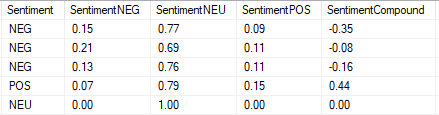
\includegraphics[scale=0.6]{sentiment_score.PNG}
\caption{Example Sentiment Classification}
\label{fig1}
\end{center}
\end{figure}

First, the comments were classified as overall positive (POS), negative (NEG), or neutral (NEU) using a new column called "Sentiment". These classifications can be seen in Figure $1$. There are many methods to do this, but after trial and error, the best method for us was to use the compound score. If the score was lower than -0.05, it was negative, if it was above 0.05, it was positive, and anything between was classified as neutral.

\subsection{Sentiment Analysis}

Sentiment Analysis is the contextual mining of text which identifies and extracts subjective information in source material. Commercial products, such as the ParallelDots API yields classification of text as positive, neutral, or negative. However, these APIs can be insufficient in such a project because the underlying methodologies are not disclosed due to their commercial nature. Further, there are usually steep limitations on the number of API calls that can be made unless one is willing to pay a premium for increased usage. Thus, we had to do some research to find an adequate tool for the sentiment analysis portion of this project. 

We found and ultimately utilized the VADER module \cite{VaderModule} in the Natural Language Toolkit (NLTK) package in Python to perform sentiment analysis on the text of all comments. The VADER module is comprised of two main components - the VADER \textbf{sentiment lexicon} and the \textbf{rule-based sentiment analysis engine}. The VADER sentiment lexicon was constructed by empirically validating the lexicon with multiple independent human judges and incorporates a "gold-standard" sentiment lexicon that is especially attuned to social media contexts. It is sensitive to both the polarity and the intensity of sentiments expressed in social media context. Notably, degree modifiers - intensifiers, booster words, or degree adverbs - impact sentiment by either increasing or decreasing the intensity. The rule-based sentiment analysis engine implements the grammatical and syntactical rules described in the VADER paper by Hutto and Gilbert \cite{VaderModule}, incorporating empirically derived quantification for the impact of each rule on the perceived intensity of sentiment in sentence-level text. 

For each JSON Object representing a Reddit comment, the comment's text will be extracted and passed to VADER's Sentiment Analyzer. The Sentiment Analyzer returns a JSON Object containing $4$ valence scores - positive, neutral, negative, and compound. The positive, neutral, and negative classifications are self-explanatory and therefore straightforward. The compound score is computed as follows: the sum of the valence scores of all words in the text, which is then normalized between $-1$ (most negative) and $1$ (most positive). This normalized, weighted metric is useful in comparing sentiment for any text. It should be noted that only compound scores in the range $(-0.05, 0.05)$ can be considered neutral.

Sentiment Analysis tools can utilize a number of different methods to achieve classification results. Some use Long Short Term Memory Neural Networks (LSTMs), which model sentences as chains of forget-remember decisions based on context. However, VADER's rule-based sentiment analysis engine uses a combination of bag of words and n-grams to achieve its classification results.

\begin{figure}[htbp]
\begin{minipage}[t]{0.45\linewidth}
    \raisebox{-0.5\height}{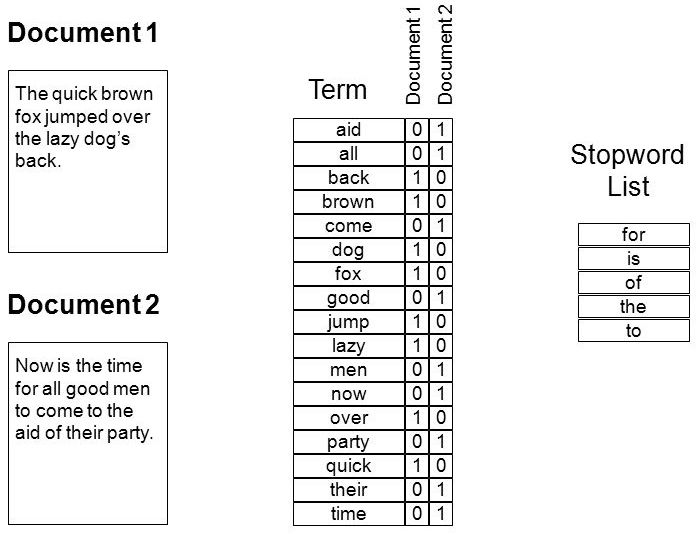
\includegraphics[width=\linewidth]{bag-of-words.jpg}}
    \caption{Simple Bag of Words Model}
    \label{f1}
\end{minipage}%
    \hfill%
\begin{minipage}[t]{0.45\linewidth}
    \raisebox{-0.5\height}{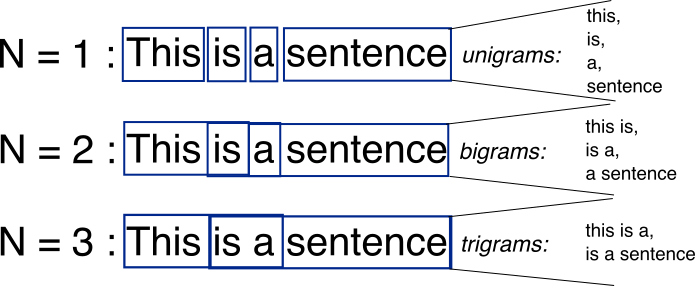
\includegraphics[width=\linewidth]{n-grams.png}}
    \caption{Simple N-gram Model}
    \label{f2}
\end{minipage} 
\end{figure}

Generally, a bag-of-words model is a representation of text that describes the occurrence of words within a document. It involves two things: a vocabulary of known words, and a measure of the presence of known words. Bag-of-words completely discards information about the order or structure of words in the document. It only tells us if a word in the known vocabulary occurs in a given document, not about the location of such a word. A simple bag-of-words model is included in Figure $2$. The intuition of this model is that documents are similar if they have similar content. Further, n-grams of text are a set of co-occurring words within a given window. They are used for a variety of different tasks, such as developing a language model or developing features for supervised Machine Learning models like Support Vector Machines, Max Entropy models, and Naive Bayes. A simple bag-of-words model is included in Figure $3$.

To help make sense of the results, multiple queries were used on the database of sentiment comments. MSSQL is quick and efficient in returning records that can be used to find trends and patterns in the data. More will be discussed in the results section, but here is a list of some example queries used for the project.

\begin{enumerate}
    \item Find how many comments were created on a given day
    \item Find out how many total words there are in all comments
    \item Find out how many comments contain the word 'trump' or 'hillary'
    \item Count the number of records from the subreddit 'worldpolitics'
    \item Find the sentiment of positive, negative, and neutral a day before and after the election
\end{enumerate}

A full query and result example are presented in Figure $4$ and Figure $5$.

\begin{figure}[!htb]
\begin{center}
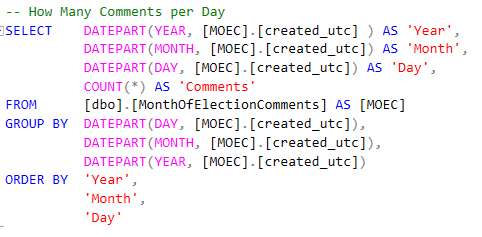
\includegraphics[scale=0.7]{example_query.PNG}
\caption{1st Example Query}
\label{fig1}
\end{center}
\end{figure}

\begin{figure}[!htb]
\begin{center}
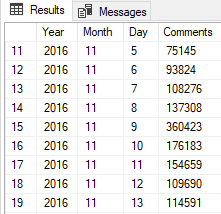
\includegraphics[scale=0.7]{example_query_result.PNG}
\caption{1st Example Query Results}
\label{fig1}
\end{center}
\end{figure}



\subsection{Emotional Analysis}
Emotional Analysis is the measuring of emotional content in textual data. It is critical when needing to quantify attitudes and feelings from unstructured text. Due to the limitations of commercial products like ParallelDots, as previously mentioned, we had to find a way to associate words and their emotions through other means.

After some research, we found the NRC Emotion Lexicon - a list of 14,182 English words and their associations with eight basic emotions (anger, fear, anticipation, trust, surprise, sadness, joy, and disgust) and two sentiments (negative and positive). An association score of $0$ means \textit{not associated} and a score of $1$ means \textit{associated}. The annotations were manually done by crowd-sourcing.

There is no doubt that this is a gross simplification of possible emotional states. On the other hand, we have to simplify emotion to gain any understanding of it and perform any form of analysis. If we use too many categories for emotion, the analyses become impossible to understand and use. Thus, we found the NRC Emotion Lexicon to be a perfect source.

Before associating emotions to the words found throughout the data set, we needed to clean and filter the comments. We did the following (in order) to clean each comment:
\begin{enumerate}
    \item Lowercase the comment
    \item Remove any URLs
    \item Remove any numbers
    \item Remove any punctuation
    \item Remove any white-space (new-line characters, tabs, etc.)
    \item Remove any stop words
    \item Perform Lemmatization
\end{enumerate}

While capitalization, punctuation, and even numbers have an effect on the emotional analysis of \textit{sentences}, they do not have an effect on our emotional analysis because we are only trying to match words with their associated emotions within the NRC Emotion Lexicon. Thus, only the words themselves have meaning to us.

The first five items were accomplished through simple string manipulation in Python. For $6$, we compared each comment to a list of 326 stop words (and, the, they, etc.) and removed any that were found. Lastly, the NLTK Python package was used to perform Lemmatization on the cleaned comment. Lemmatization, in linguistics, is the process of grouping together the different inflected forms of a word so they can be analyzed as a single time. For example, the word \textit{dogs} would become \textit{dog}, and the word \textit{cacti} would become \textit{cactus}.

After every comment is cleaned and filtered, we tokenize them into separate words then filter to keep those that have associated emotions within the NRC Emotion Lexicon, all while keeping count. The results are then put into JSON objects to be read and analyzed later.

% ------------------------------------

\section{7 EVALUATION}
We will provide both evaluations of our approach and results based on each of the objectives listed in the Objectives section.

\subsection{Data Acquisition and Cleaning}

The iterative approach to cleaning the data set proved useful because we were able to incrementally save versions of the data set and subsets of the data set as needed. The reason this was deemed a valid approach instead of producing a single data set is that the different versions of the data set could be used for different parts of the analysis. For example, all of the comments were split into separate files for each day, including the day of the election. This way, all analysis on comments for a single day, such as the day of the election, could be done on a small subset of the overall data set, decreasing overall processing time.

Overall, it took approximately $4$ hours to initially filter the original compressed data sets and output the modified October and November data sets before combining them. The combined, filtered data set based on the process described in the approach section yielded a JSON data file of $3,299,624$ objects that was $1.08$ gigabytes.

\begin{figure}[htbp]
\begin{minipage}[t]{0.45\linewidth}
    \raisebox{-0.5\height}{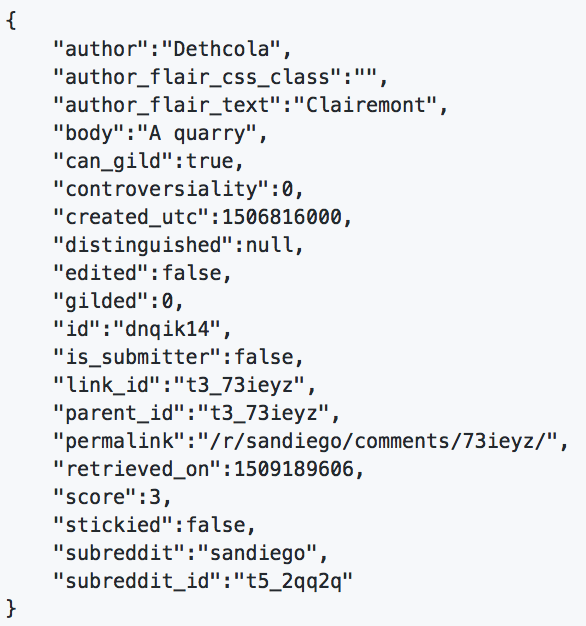
\includegraphics[width=\linewidth]{Original-Dataset-Attributes.png}}
    \caption{Original Data Set Attributes}
    \label{f1}
\end{minipage}%
    \hfill%
\begin{minipage}[t]{0.45\linewidth}
    \raisebox{-0.5\height}{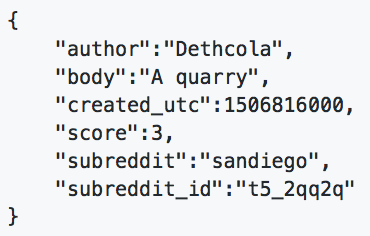
\includegraphics[width=\linewidth]{Filtered-Dataset-Attributes.png}}
    \caption{Filtered Data Set Attributes}
    \label{f2}
\end{minipage} 
\end{figure}

Figure $6$ shows the all of the attributes of the original data set. It can be seen that the attributes are verbose but not all useful in this analysis. For example, there would not be any particular use for author\_flair\_text. Thus, during the cleaning part of Objective $1$, we made sure to remove such attributes. Figure $7$ shows the attributes ultimately chosen for this project. Each was chosen for a specific reason. Namely, the body will be the main piece used for the sentiment and emotional analysis. The author attribute is unique and was useful to determine how often people post a comment.


\subsection{Sentiment Analysis}

\begin{figure}[!htb]
\begin{center}
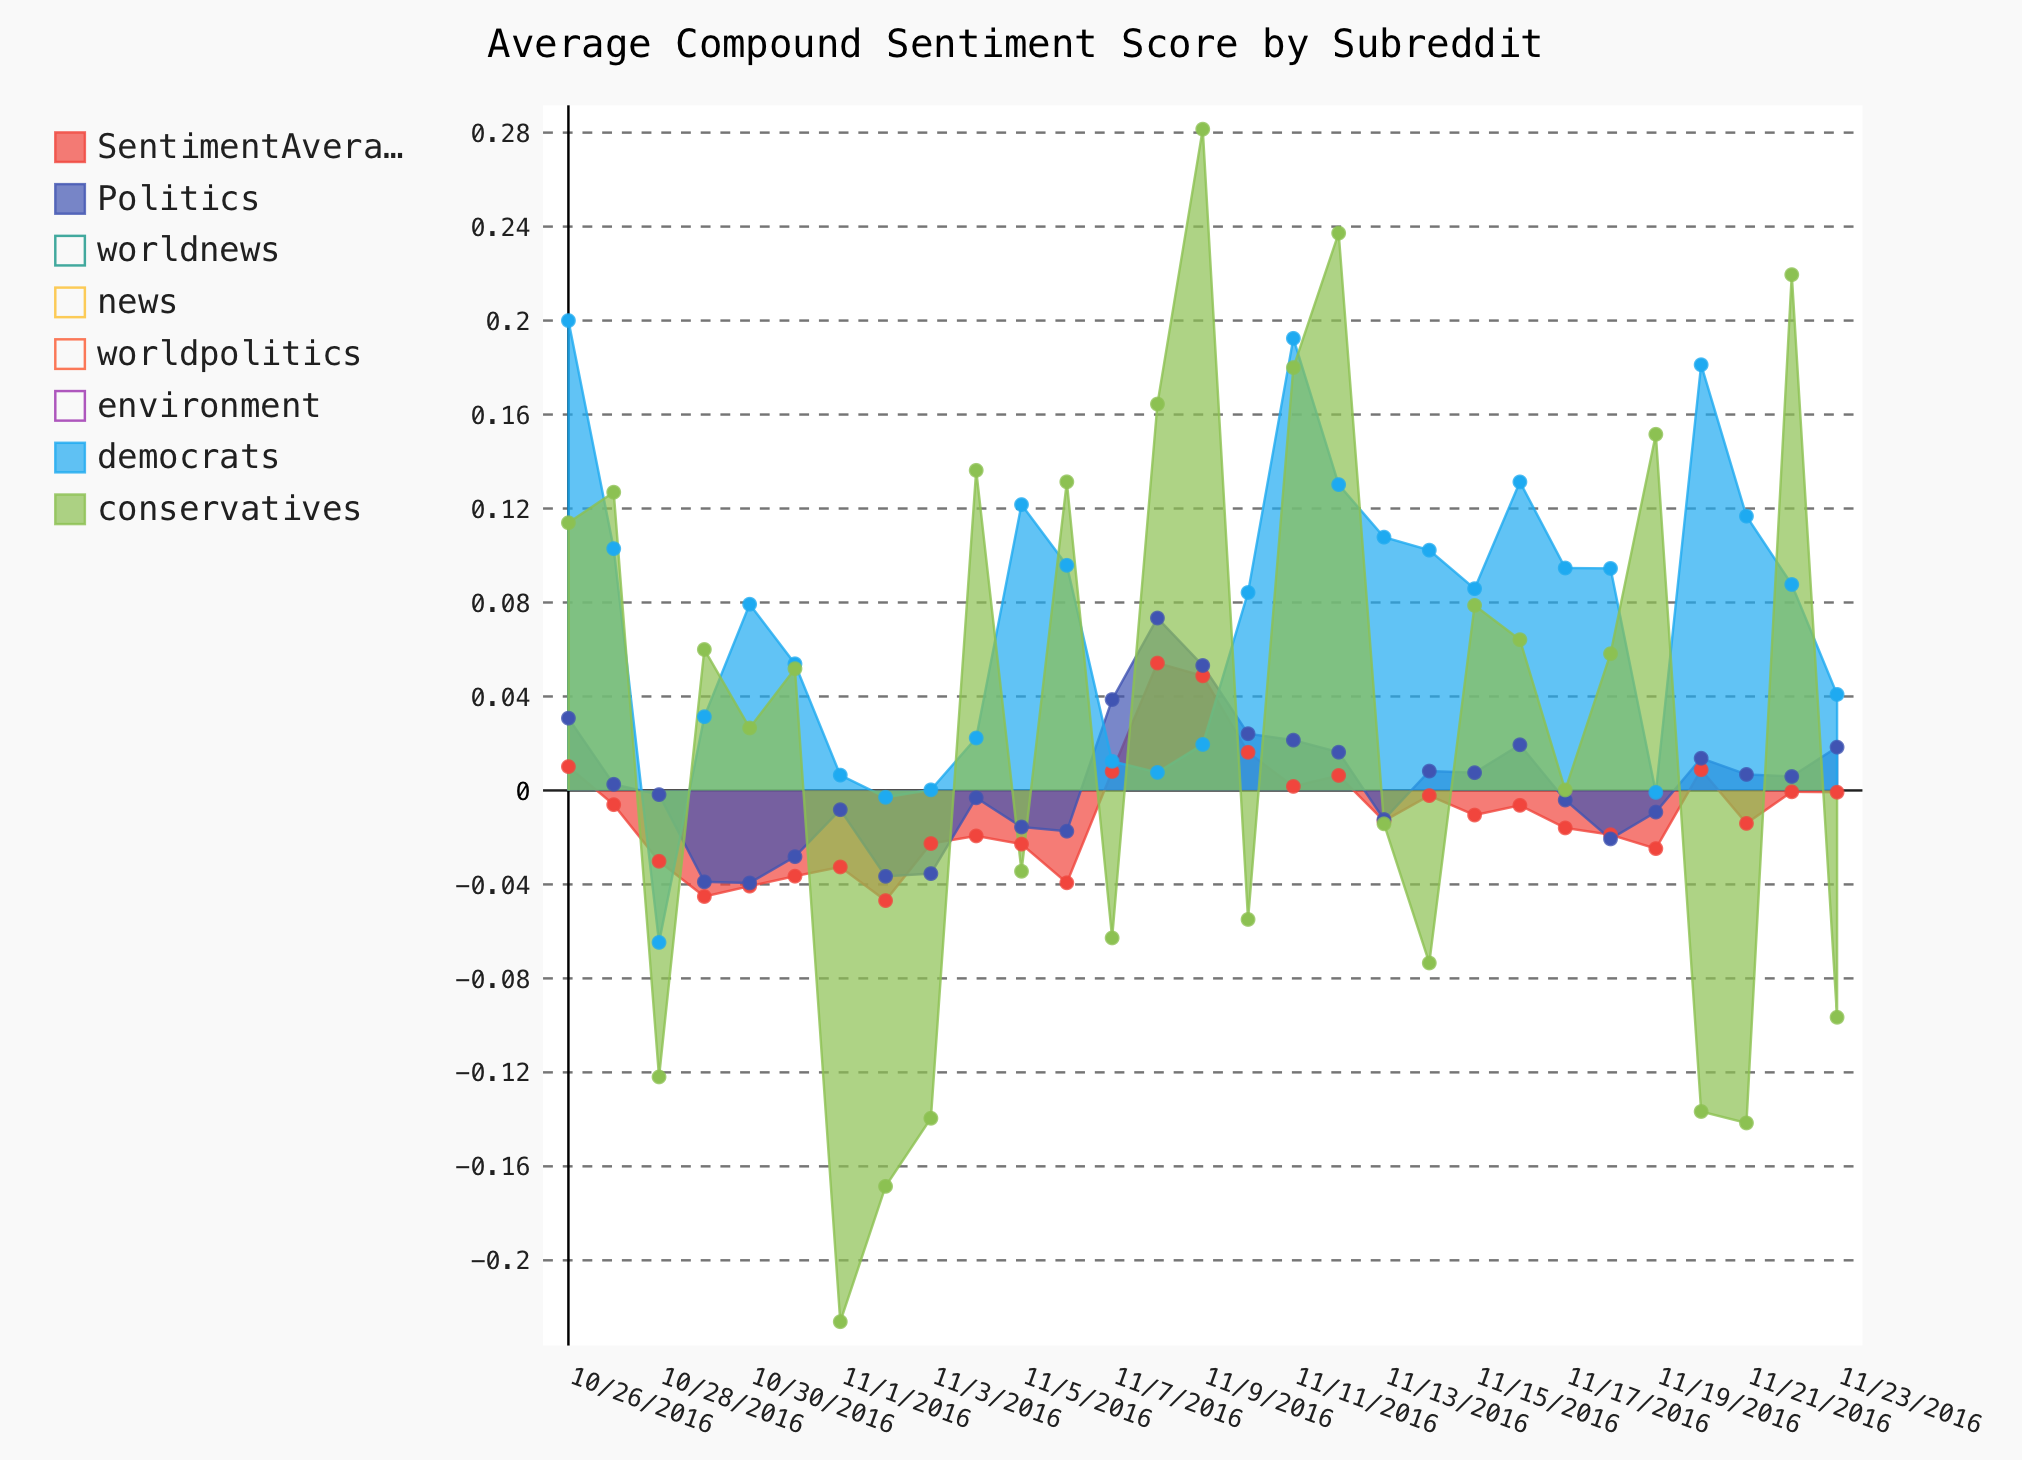
\includegraphics[scale=0.2]{avg-sentiment-stacked.png}
\caption{Overall Average Sentiment}
\label{fig1}
\end{center}
\end{figure}

Figure $8$ shows the average sentiment for the duration of the two week before and after period considered. As expected, the average sentiment for all subreddits over the period contains far less variance than any single subreddit considered. Interestingly enough, the Politics subreddit is highly correlated with the average sentiment for all subreddits. As expected, the democrats and conservatives subreddits have a high amount of variance in the average sentiment of their comments, especially around the day of the election. An unexpected result was that the environment subreddit contained seemingly random variation in the polarity of its sentiment. This result seemed strange, so we wanted to do some further investigation. 

\begin{figure}[!htb]
\begin{center}
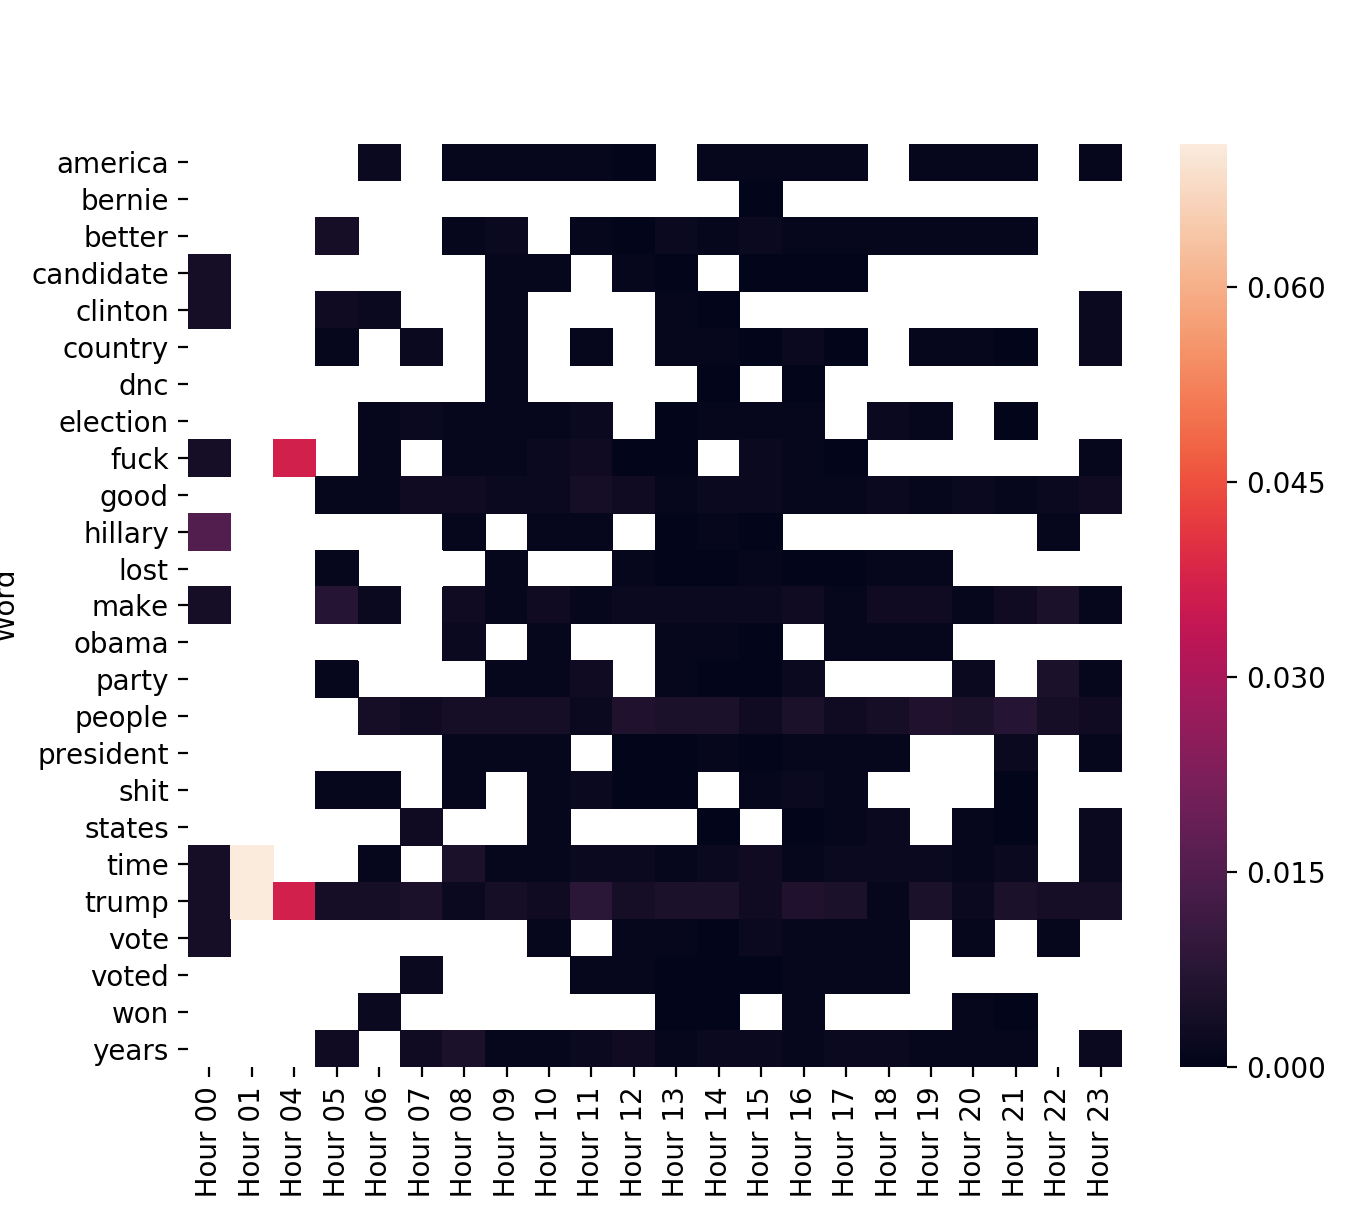
\includegraphics[scale=0.4]{day-of-election-environment.png}
\caption{Day of Election Environment Subreddit Heat Map}
\label{fig1}
\end{center}
\end{figure}

Figure $9$ shows a heat map of the occurrence of the most popular words found among all subreddits in the environment subreddit on the day of the election. The figure shows that most popular words are not present. Thus, we concluded that the variation in sentiment in the environment subreddit was less correlated with the events of the election than other subreddits. From the data available, we are unsure of the cause of the variation in sentiment.

\begin{figure}[!htb]
\begin{center}
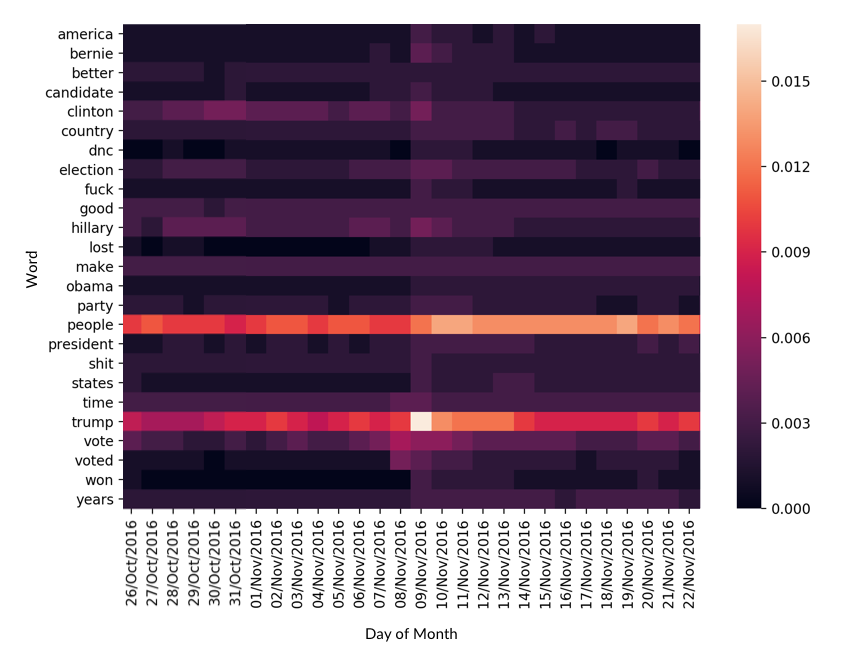
\includegraphics[scale=0.3]{full-month-heatmap.png}
\caption{Overall Most Popular Words Heat Map}
\label{fig1}
\end{center}
\end{figure}

Figure $10$ shows a heat map of the occurrence of the most popular words found among all subreddits throughout all comments over the course of the two weeks before and after the day of the election. The occurrence of the words are measured as the percentage of the number of occurrences of a specific word out of all the words found on any given day. It is therefore expected that the occurrence percentage of any word found would be rather low. However, we can see that the most popular words throughout the course of the period are \textit{people} and \textit{Trump}. Most notably, the occurrence of the \textit{Trump} peaks on November $9$th, which was the day after the election. We suspect the reason for this was the unexpected election result combined with the delay of election results until early that morning.

\begin{figure}[!htb]
\begin{center}
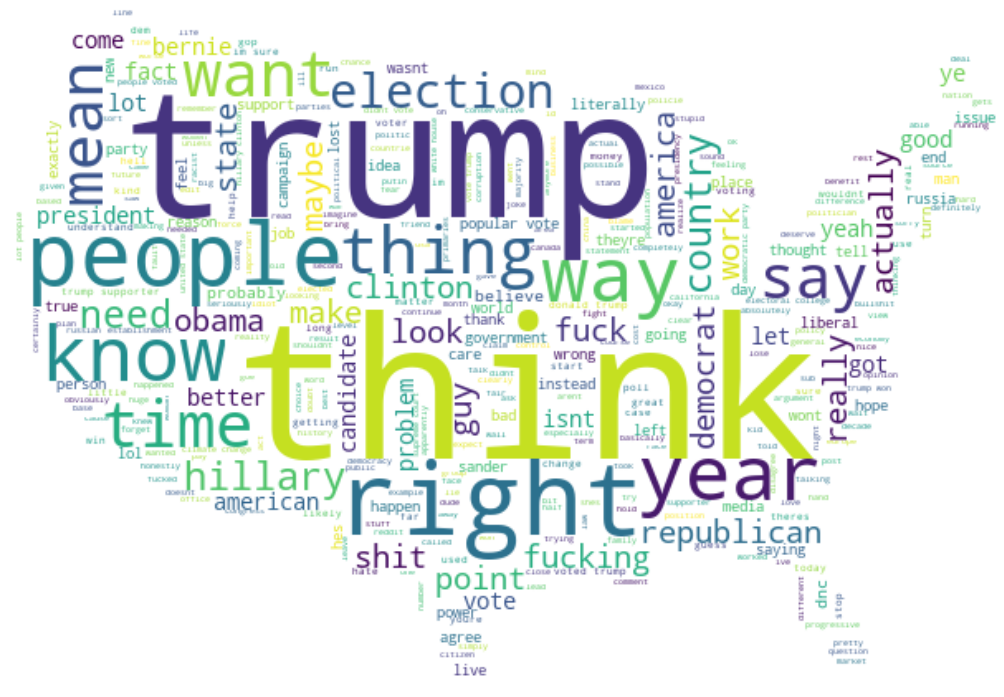
\includegraphics[scale=0.5]{day-of-comments-mask.png}
\caption{Day of Election Word Cloud}
\label{fig1}
\end{center}
\end{figure}

Figure $11$ shows a word cloud generated from the text of comments on the day of the election masked by the shape of the United States. Word clouds are a useful visualization for showing the relative occurrence of words in text in comparison to other words found. Not surprisingly, we see that Trump, think, and people are among the words that occur the most. Less prominent but still present are words like Hillary, Obama, republican, and election. There is not much additional information that can be derived from this visualization.

\begin{figure}[!htb]
\begin{center}
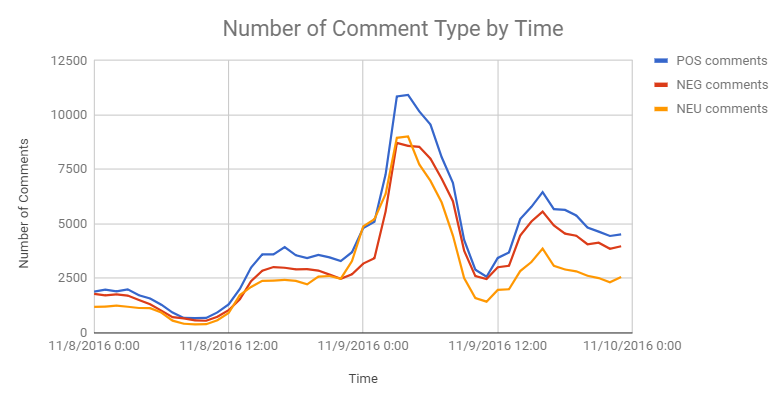
\includegraphics[scale=0.4]{comment_count_sentiment.PNG}
\caption{Number of Comment Type by Time}
\label{fig1}
\end{center}
\end{figure}

Figure $12$ shows the count of the comments by each sentiment from midnight to midnight between November $8$ and $11$, $2016$. To find these results, the database was queried to find the number of comments by each sentiment type. Before the election took place, the percent of comment types were roughly equal at ~33\% for each type. When the election starts, the spread grows, with positive comments having the greatest count, followed by negative, and then neutral. At the peak number of comments, positive sentiment remains on time. After the election, the spread changes to roughly ~75\% positive or negative, and 25\% neutral. It is interesting to compare the spread before and after the election. We suspect that peoples comments were more opinionated after the election, and therefore used a more positive or negative sentiment.

\begin{figure}[!htb]
\begin{center}
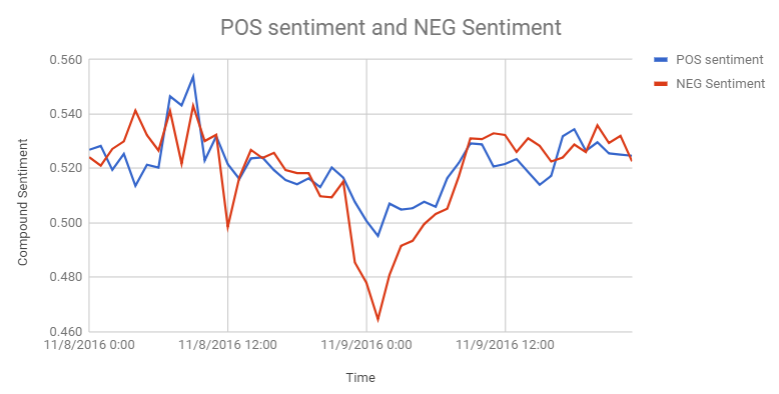
\includegraphics[scale=0.4]{pos_neg_sentiment.PNG}
\caption{Number of Comment Type by Time}
\label{fig1}
\end{center}
\end{figure}

Figure $13$ shows the positive and negative sentiment from midnight to midnight between November $8$ and $11$, $2016$. To find these results, the database was queried to find the average sentiment based on positive and negative comments only. The absolute value of the negative comments was taken to better see the difference between positive and negative. Neutral comments were not used as they brought the overall average closer to $0$, and that wasn't helpful when looking for large swings in sentiment. At the start of the election and after the election, the overall sentiment average for both positive and negative was similar, between +/-0.520 and +/-0.540. During the election the average sentiment slightly dips for positive sentiment (+.510) and drops sharply for the negative sentiment (-.460). This result is interesting because it goes against what we previously had thought we had found. When querying the data based on overall sentiment, it appears that the number of positive comment sentiment grows during the election. However, based on this data, a better way to frame it may be: The overall sentiment of negative comments decreases, thus making it look like positive comment sentiment was increasing.


\begin{figure}[!htb]
\begin{center}
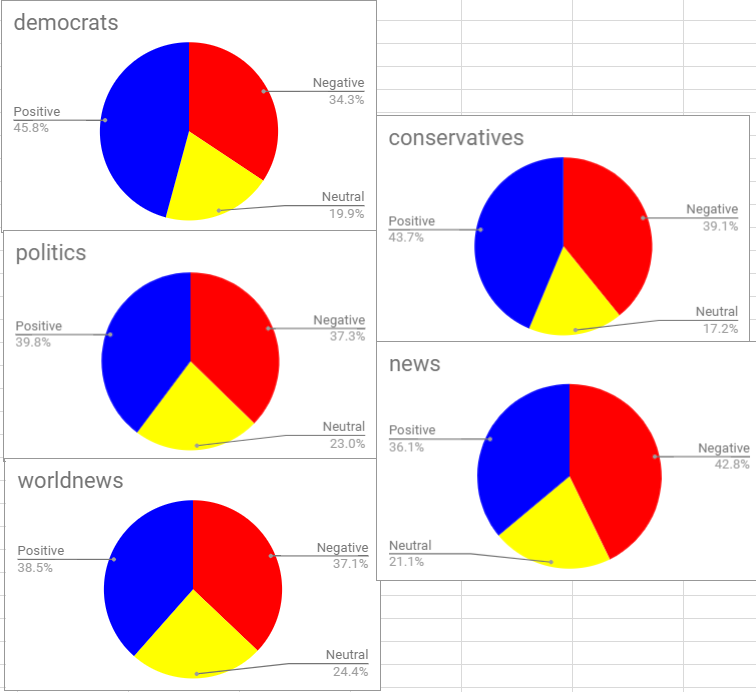
\includegraphics[scale=0.4]{sentiment_subreddit_vertical.PNG}
\caption{Number of Comment Type by Time}
\label{fig1}
\end{center}
\end{figure}
\par
Figure $14$ shows the positive, negative, and neutral percentage splits for five selected subreddits: democrats, conservatives, politics, news, and worldnews. The comment types were counted and averaged in order to obtain these scores. Observing all five pie charts, the trends are similar throughout the subreddits. The positive comments are equal or greater in proportion compared to the negative comments, and the neutral comments have smallest percent. The most positive subreddit based on this analysis was democrats, and the most negative was news. This type of breakdown is interesting to observe as it can provide further information about a subreddit. For example, if a subreddit claims to be "non-bias" sentiment analysis can be done during a certain time period to hopefully show that the comments have a majority of neutral comments, or at least an even split between positive and negative comments.


\subsection{Emotional Analysis}
We found over 117 million words, in total. After cleaning, we found 443,725 unique words. Out of the 14,182 words within the NRC Emotion Lexicon dataset, we were able to match with 8,215 of them.

\begin{figure}[!htb]
\begin{center}
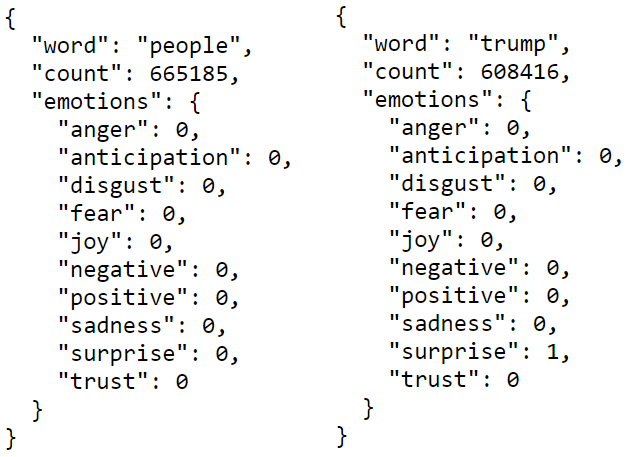
\includegraphics[scale=0.9]{topTwoWordsWithEmotion.png}
\caption{JSON Objects of Matched Words}
\label{fig1}
\end{center}
\end{figure}

Figure $15$ shows the two most-said words throughout the entire data set, including their counts and associated emotions.

Having a count of 665,185, we found \textit{people} to occur the most. However, even though \textit{people} is in the NRC Emotion Lexicon, it has the value $0$ for every emotion, meaning that it doesn't necessarily fit under any of the eight basic emotions or the two sentiments, and the word \textit{people} won't have an impact on our emotional analysis.

Having a count of 608,416, we found \textit{trump} to occur the second most. Unlike Hillary, \textit{trump} is both a noun and a verb, which happens to be included in the NRC Emotion Lexicon. This slightly skews our results, later visualized in Figure $18$ and discussed thereafter.

\begin{figure}[!htb]
\begin{center}
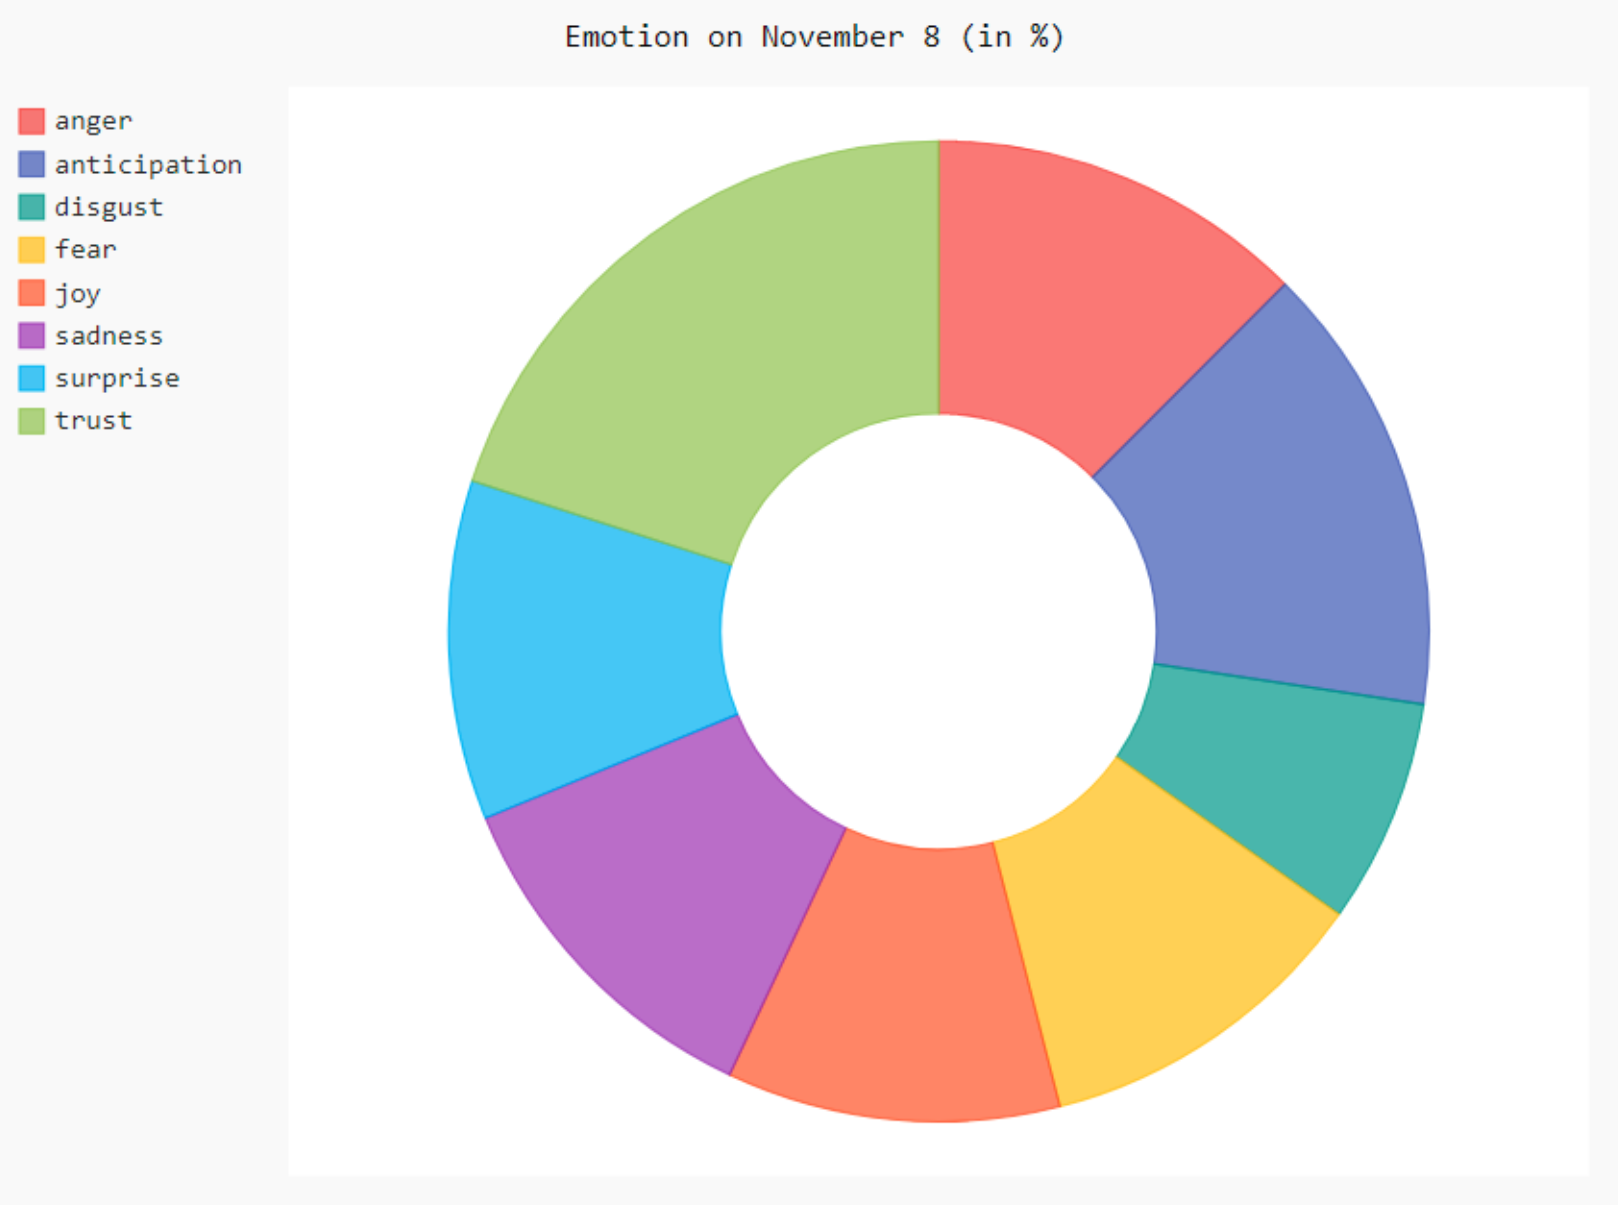
\includegraphics[scale=0.38]{emotion-on-nov-8.PNG}
\caption{Emotion on November 8}
\label{fig1}
\end{center}
\end{figure}

Figure $16$ is a pie-chart representing the amount of each emotion shown on November $8$th. This was done by summing up the count of words in each category of emotion and comparing them to each other. As seen in the figure, \textit{trust} was the most prevalent emotion on the day of the election. On the other hand, \textit{disgust} was the least prevalent. This is an interesting result, as we'll later see that \textit{disgust} was the emotion that grew the most preceding the election.

\begin{figure}[!htb]
\begin{center}
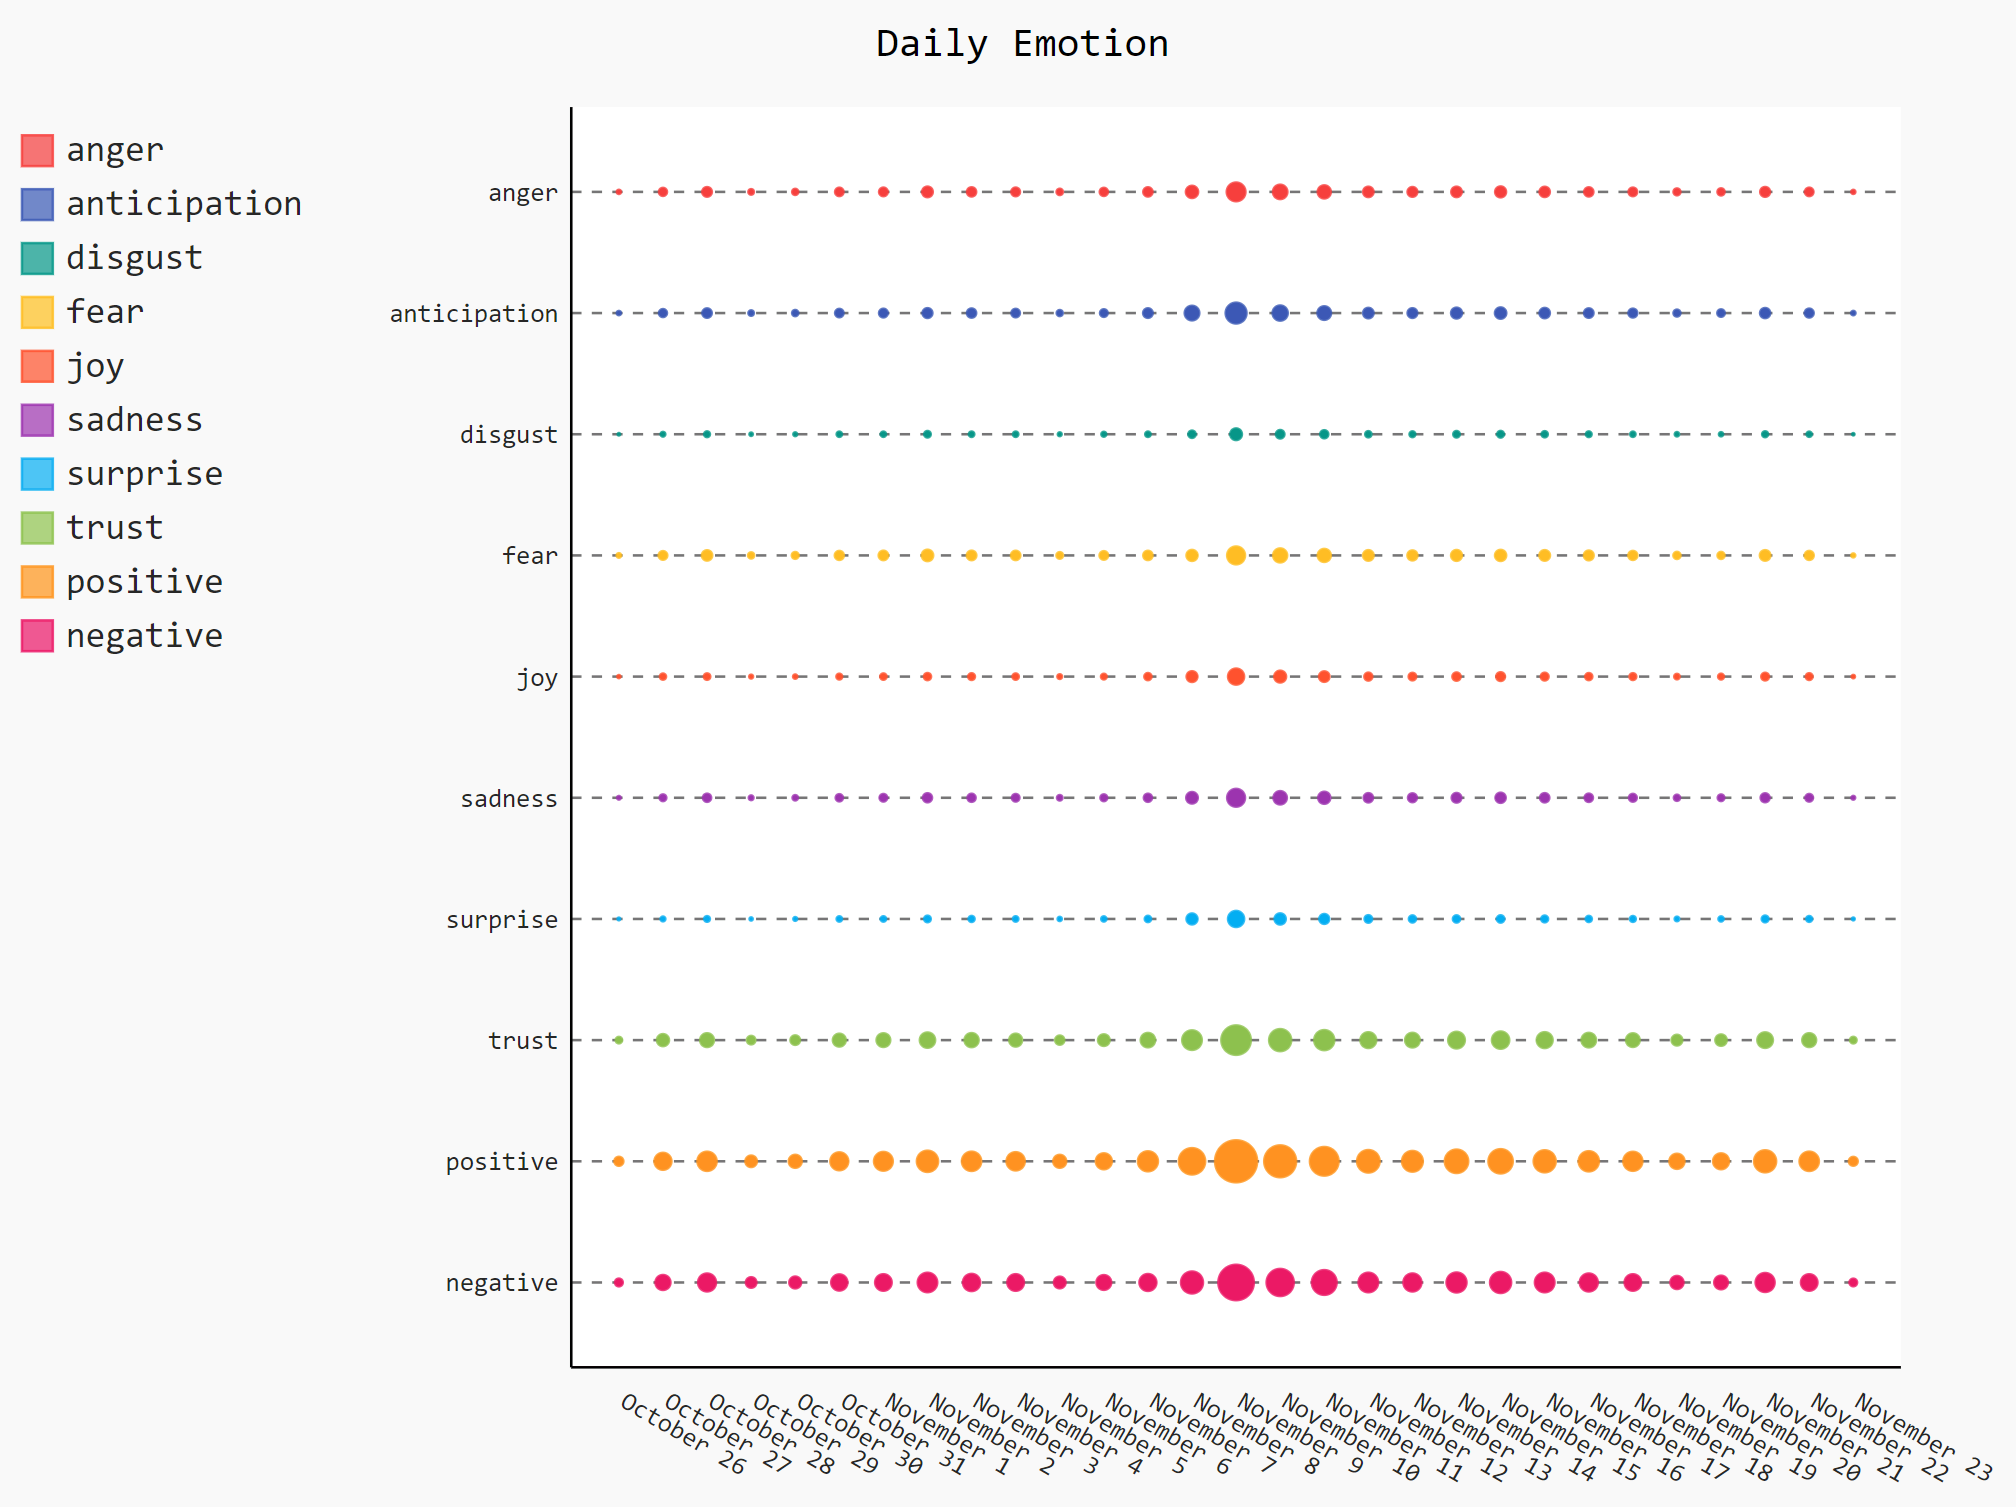
\includegraphics[scale=0.3]{daily-emotion-all.PNG}
\caption{Daily Emotion}
\label{fig1}
\end{center}
\end{figure}

Figure $17$ shows the daily count for each emotion on each day, with the size of the dots representing the count of each emotion. Thus, a larger dot means that the emotion was quite prevalent that day. Although there seems to be a general increase in each emotion before the election, and a general decrease in each emotion after the election, this doesn't necessarily tell us too much. Due to the coverage of the event, it is not odd to see larger dots around the day of the election, as more people would be posting comments. However, we can use this graph, and the previous one, as a references while looking at the next figure to formulate some interesting conclusions regarding emotion.

\begin{figure}[!htb]
\begin{center}
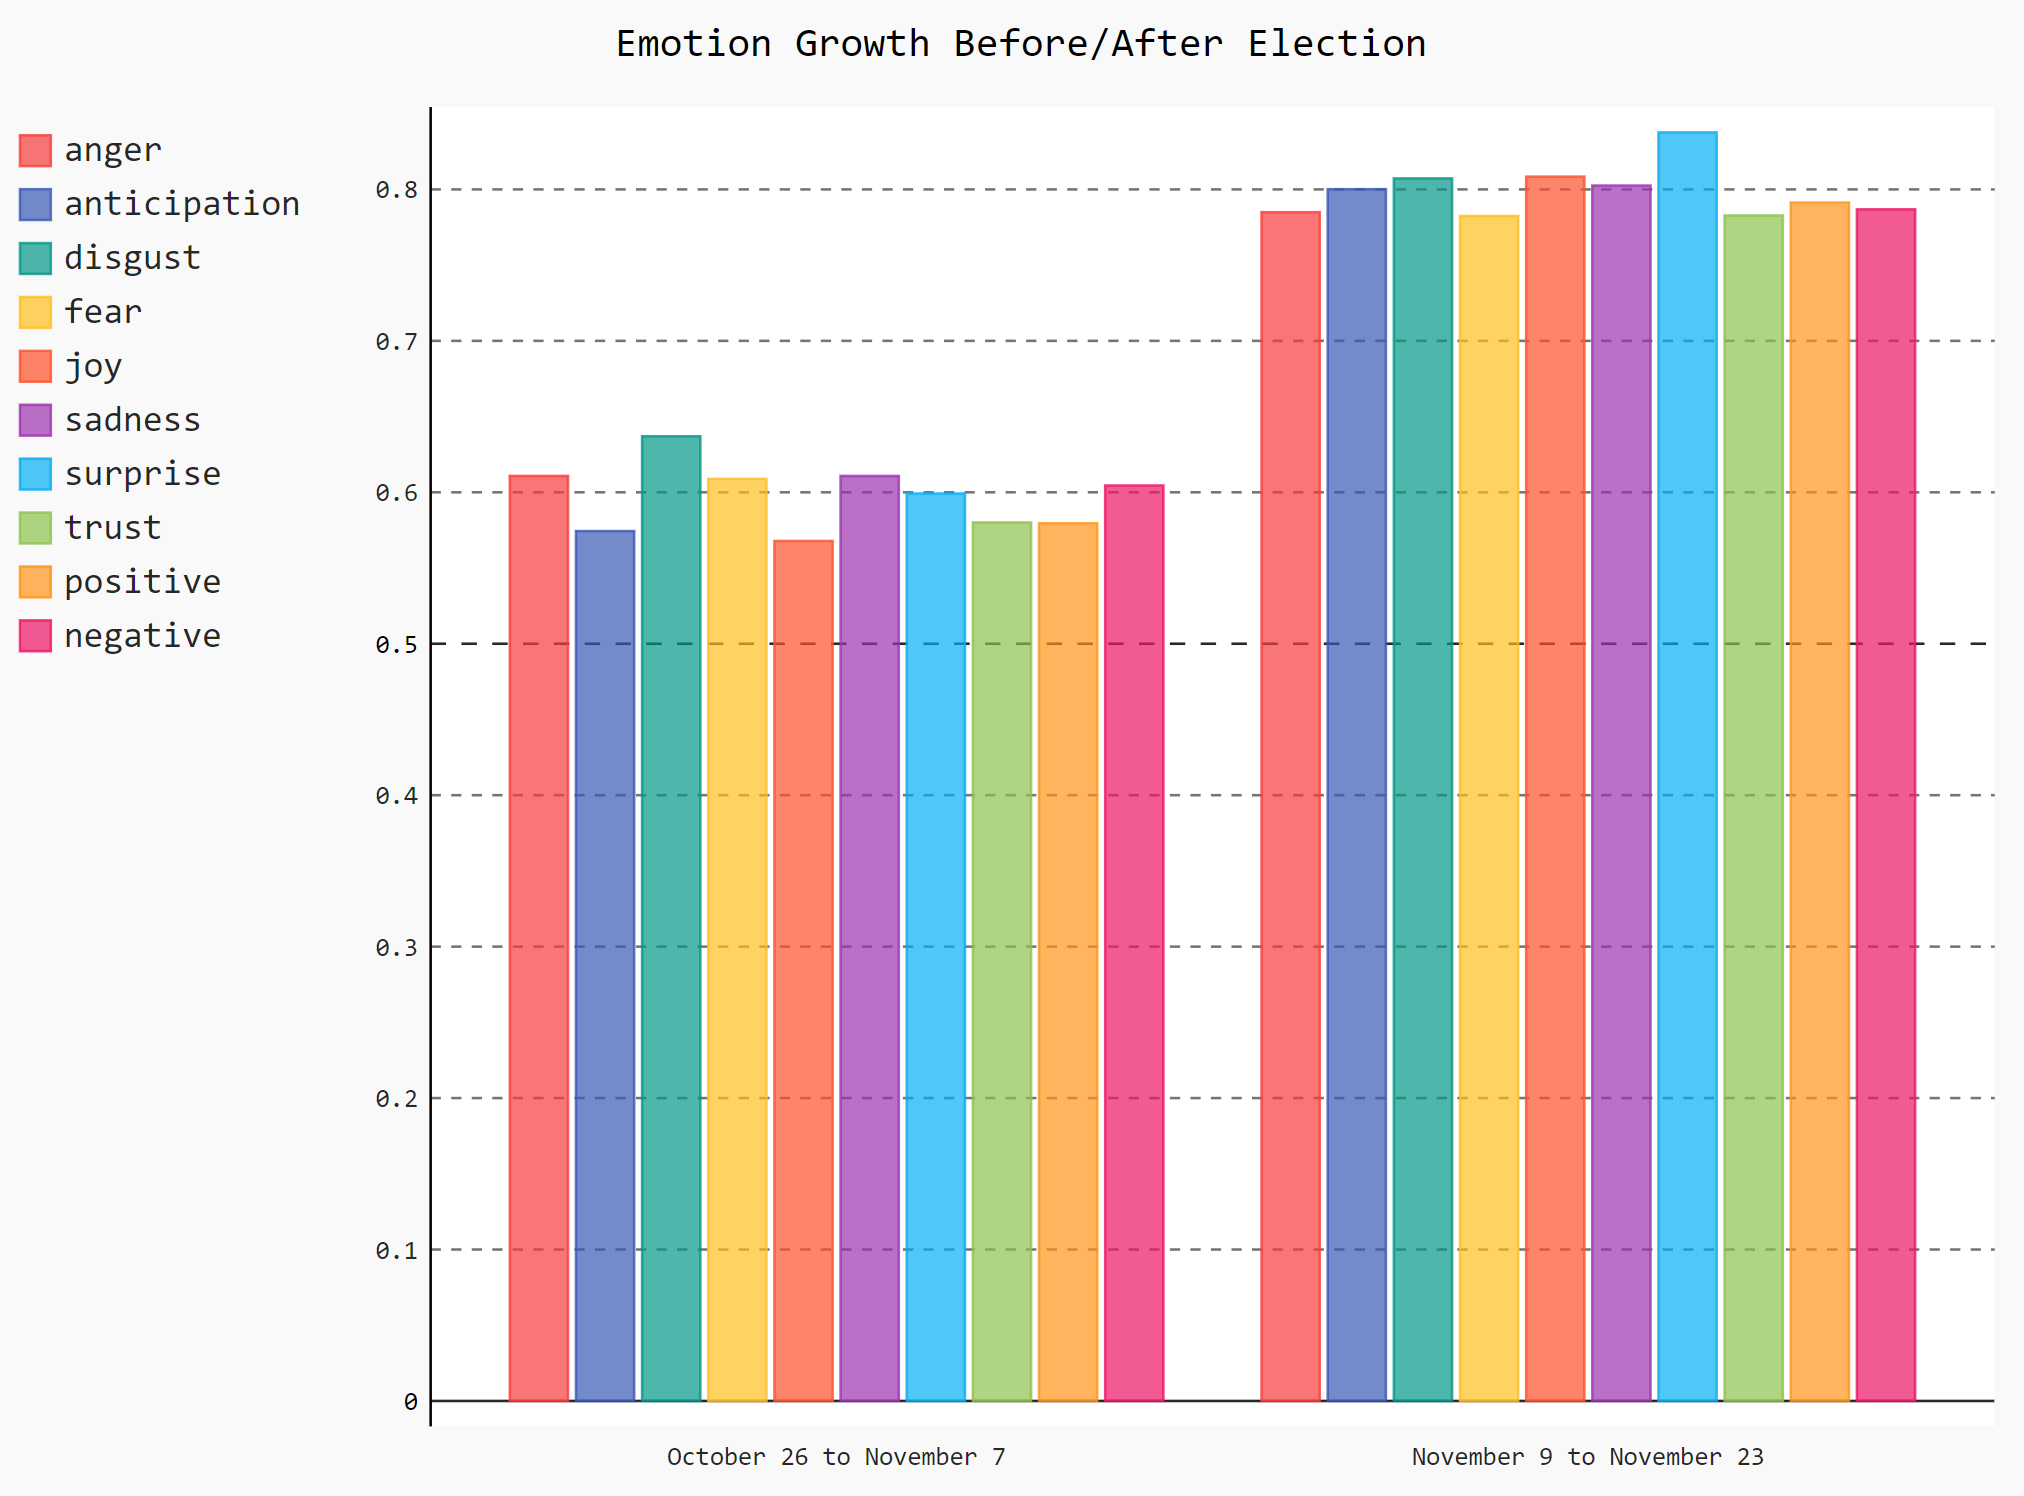
\includegraphics[scale=0.3]{emotion-growth-ba.PNG}
\caption{Emotion Growth Before/After Election}
\label{fig1}
\end{center}
\end{figure}

Figure $18$ shows the net change in each emotion from October $26$th to November $7$th, the two weeks before the election, and from November $9$th to November $23$rd, the two weeks after the election.

As previously mentioned from Figure $17$, each emotion generally increased preceding the election. Thus, the left side shows the net \textit{increase} in each emotion. Interestingly enough, \textit{disgust} was the emotion that increased the most with a net change of 64 percent. Although it increased the most out of every emotion, it must not have been that prevalent before because Figure $16$ shows it to be the least prevalent emotion on the day of the election.

As previously mentioned from Figure $17$, each emotion generally decreased following the election. Thus, the right side shows the net \textit{decrease} in each emotion. The emotion, \textit{fear}, decreased the least with a net change of 78 percent. Thus, it remained prevalent within the comments more than the other emotions after the election. We can see that \textit{surprise} decreased the most with a net change of 84 percent. However, recall that the word \textit{trump} was the second-most occurring word, associating with the emotion \textit{surprise}. Thus, we can't exactly determine if the emotion actually decreased, or if Trump was just talked about less after the election was over.

% ------------------------------------

\section{8 IMPLEMENTATION PLAN AND TIMELINE}

In order to successfully complete this project in a timely manner, we created the following implementation timeline. There were points along the way where a task took longer than expected, but we were able to successfully complete the project. It is worth noting that the completion of the second and the third objectives were the most time intensive. \\

\noindent
The presentation task refers to an actual class presentation to the Spring $2018$ section of CSCE $474$ at the University of Nebraska-Lincoln taught by Dr. Ashok Samal. The purpose is to relay the information of this report in an easy-to-understand manner.

\begin{center}
\begin{tabular}{ | l | c | } 
\hline
\textbf{Task} & \textbf{Date} \\ 
\hline
Completion of first objective &  March $30$ \\ 
\hline
Completion of second objective & April $9$ \\ 
\hline
Completion of third objective & April $16$ \\ 
 \hline
Finalize analysis and presentation & April $16$ to April $25$ \\ 
\hline
Presentation & April $25$ \\
\hline
Final report for this project & May $1$ \\ 
\hline
\end{tabular}
\end{center}

\footnotesize
\bibliographystyle{IEEEtran}
\bibliography{reddit-sa-bibliography}

\end{document}
